\ylDisplay{Kosmosejaam} % Ülesande nimi
{Oleg Košik} % Autor
{lõppvoor} % Voor
{2005} % Aasta
{G 9} % Ülesande nr.
{6} % Raskustase
{
% Teema: Taevamehaanika
\ifStatement
Joonisel on toodud ringorbiidil liikuva rahvusvahelise kosmosejaama trajektoor maapinna kohal (Maa keskpunktist kosmosejaamani tõmmatud sirge ja maapinna lõikepunkti jälg). Hinnake selle abil kosmosejaama kõrgust maapinnast. Maa raadius $R = \SI{6380}{km}$, raskuskiirendus maapinnal $g = \SI{9,8}{m/s^2}$.

\begin{center}
	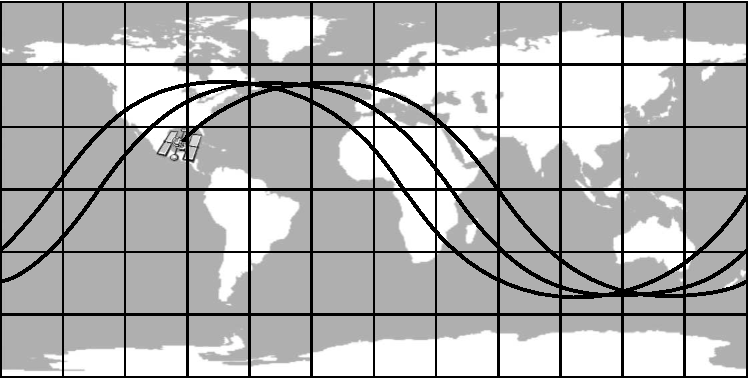
\includegraphics[width=\linewidth]{2005-v3g-09-yl}
\end{center}
\fi


\ifHint
Kosmosejaama trajektoori nihked on põhjustatud maa pöörlemisest ümber oma telje, kusjuures ühele ööpäevale vastava kosmosejaama nihke ja Maa ekvaatori pikkuse suhe on otseses sõltuvuses kosmosejaama ja maa pöörlemise nurkkiiruste suhtega.
\fi


\ifSolution
Maa pöörlemise tõttu ümber oma telje tekivad trajektoori nihked. Mõõdame nihke pikkuse ekvaatoril $\Delta l$ ning ekvaatori pikkuse (ehk kogu kaardi laiuse) $l$. Nende suhe määrab kosmosejaama nurkkiiruse $\omega_J$ ja maa pöörlemise nurkkiiruse $\omega_M$ suhte:
\[
\alpha=\frac{l}{\Delta l}=\frac{\omega_{J}}{\omega_{M}} \approx \num{15,7}.
\]
Arvestades, et maa pöörlemise nurkkiirus on $\omega_M = 2\pi /T$, kus $T$ on ööpäeva pikkus ehk \SI{86400}{s}, leiame
\[
\omega_J = \alpha \omega_M = \frac{2\pi\alpha}{T}.
\]
Kosmosejaamale mõjuv gravitatsioonijõud määrab kesktõmbekiirenduse:
\[
m g^{\prime}= m\omega_J^2 r = m \omega_{J}^{2}(R+h),
\]
kus $g'$ on raskuskiirendus kõrgusel $h$ maapinnast. Gravitatsiooniseadusest teame, et raskuskiirendus on pöördvõrdeline kauguse ruuduga, millest
\[
g^{\prime}= g\left(\frac{R}{r}\right)^2 = g\left(\frac{R}{R+h}\right)^{2}.
\]
Kombineerides kaks viimast võrrandit, saame
\[
\omega_{J}^{2}(R+h)=g\left(\frac{R}{R+h}\right)^{2},
\]
kust ostitav kõrgus on
\[
h=\sqrt[3]{\frac{g R^{2}}{\omega_{J}^{2}}}-R=\sqrt[3]{\frac{g R^{2} T^{2}}{4 \pi^{2} \alpha^{2}}}-R \approx \SI{359}{km}.
\]

\emph{Märkus}. Tegelik kõrgus varieerub \num{350} ja \SI{365}{km} vahel (Maa raadius ei ole kõikjal ühesugune). Siin $\alpha$ väärtus oli mõõdetud suhteliselt täpsete arvutigraafika vahenditega, joonlauga joonise mõõtmise korral esinevate ebatäpsuste tõttu võib vastus erineda tegelikust kuni \num{200} kilomeetri võrra. 
\fi
}